%%%%%%%%%%%%%%%%%%%%%%%%%%%%%%%%%%%%%%%%%
% LaTeX Template
% http://www.LaTeXTemplates.com
%
% Original author:
% Linux and Unix Users Group at Virginia Tech Wiki 
% (https://vtluug.org/wiki/Example_LaTeX_chem_lab_report)
%
% License:
% CC BY-NC-SA 3.0 (http://creativecommons.org/licenses/by-nc-sa/3.0/)
%
%%%%%%%%%%%%%%%%%%%%%%%%%%%%%%%%%%%%%%%%%

%----------------------------------------------------------------------------------------
%	PACKAGES AND DOCUMENT CONFIGURATIONS
%----------------------------------------------------------------------------------------

\documentclass[12pt]{article}
\usepackage{geometry} % Pour passer au format A4
\geometry{hmargin=1cm, vmargin=1cm} % 

\usepackage{graphicx} % Required for including pictures
\usepackage{float} % 

%Français
\usepackage[T1]{fontenc} 
\usepackage[english,francais]{babel}
\usepackage[utf8]{inputenc}
\usepackage{eurosym}
\usepackage{lmodern}
\usepackage{url}
\usepackage{multicol}

%Maths
\usepackage{amsmath,amsfonts,amssymb,amsthm}
%\usepackage[linesnumbered, ruled, vlined]{algorithm2e}
%\SetAlFnt{\small\sffamily}

%Autres
\linespread{1} % Line spacing
\setlength\parindent{0pt} % Removes all indentation from paragraphs

\renewcommand{\labelenumi}{\alph{enumi}.} % 

\newcommand{\horrule}[1]{\rule{\linewidth}{#1}} % Create horizontal rule command with 1 argument of height

\pagestyle{empty}
%----------------------------------------------------------------------------------------
%	DOCUMENT INFORMATION
%----------------------------------------------------------------------------------------
\begin{document}

%\maketitle % Insert the title, author and date

\textbf{Nom(s), Prénom(s) :}\\
\textit{Je choisis un nombre $x$ entre 1 et 9}. $x = $


\begin{figure}[H]
  \centering
  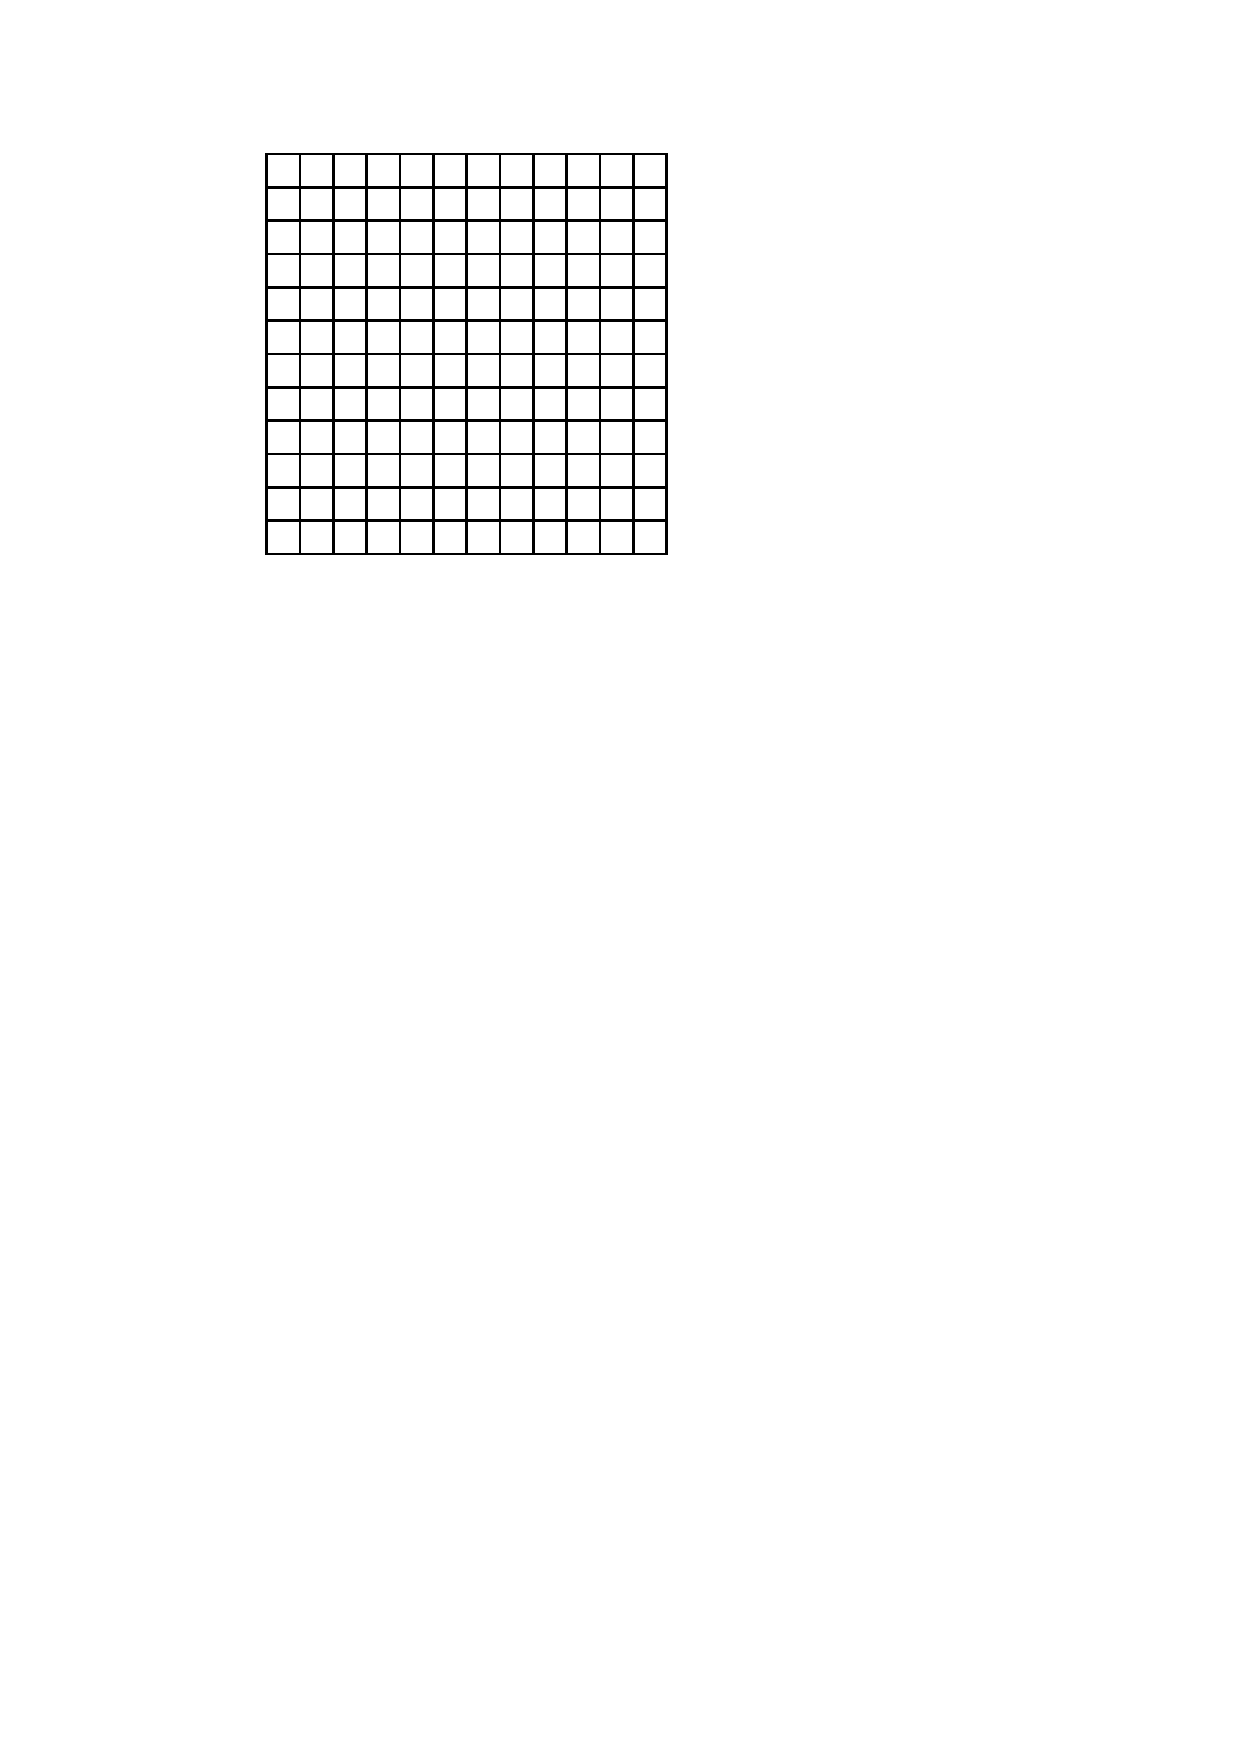
\includegraphics[width=0.7\linewidth]{sources/1/grille-dm.pdf}
\end{figure}

\horrule{1px}

\begin{enumerate}
\item[1.] Tracer un carrés $ABCD$ de côté 10. 
\item[2a.] Placer $M$ sur $[AB]$ tel que $AM =  x = $\\
Tracer la perpendiculaire à $(AB)$ passant par $M$.
\item[2b.] Placer $N$ sur $[AD]$ tel que $AN = 10 - x = 10 - \phantom{azer} = \phantom{azer}$\\
Tracer la perpendiculaire à $(AN)$ passant par $N$.
\item[3.] Placer $P$ le point d'intersection de ces deux droites. Placer $X$ le point d'intersection  des droites $(NP)$ et $(BC)$. Placer $Y$ le point d'intersection des droites $(MP)$ et $(DC)$\\
Tracer les segments $[NP]$ et $[PC]$.
\begin{multicols}{2}
\item[4.] Colorier :
	\begin{itemize}
	\item Gris  : carrés $NPYD$ et $MBXP$.
	\item Jaune : triangle $AMN$.
	\item Rouge : triangle $MPN$.
	\item Vert  : triangle $PXC$.
	\item Bleu  : triangle $PCY$
	\end{itemize}

\item[5.] Calculs d'aire. \\ \textit{( utiliser la nottion carré. )}
	\begin{itemize}
	\item Aire de ABCD = $\mathbb{A}_{ABCD} =$   
	\item Aire de MBXP = $\mathbb{A}_1 =$   
	\item Aire de ABCD = $\mathbb{A}_2 =$   
	\item $\mathbb{A}_1 + \mathbb{A}_2 =$
	\end{itemize}

\end{multicols}
\end{enumerate}

\newpage
\

\begin{figure}[H]
  \centering
  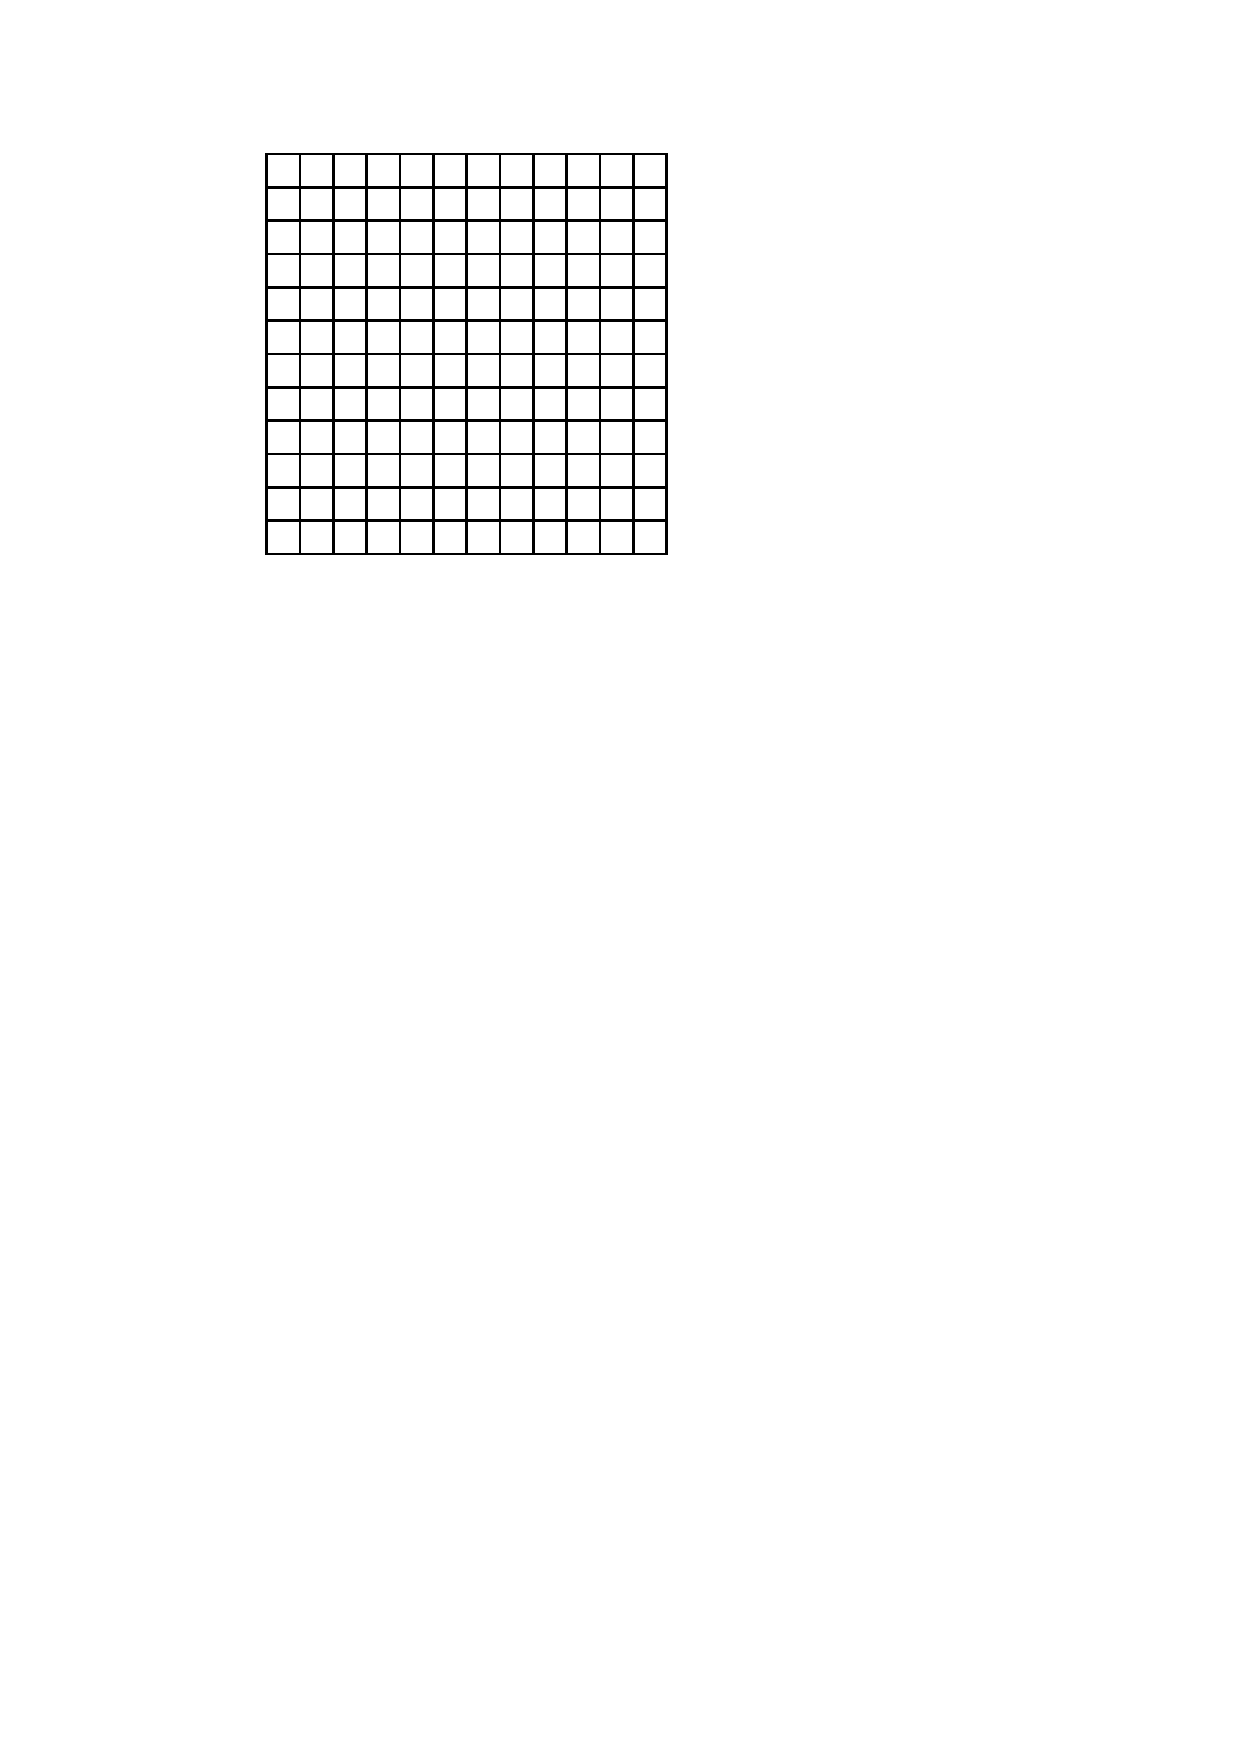
\includegraphics[width=0.7\linewidth]{sources/1/grille-dm.pdf}
\end{figure}

\horrule{1px}

\begin{enumerate}
\item[1.] Tracer un carrés $ABCD$ de côté 10. 
\item[2a.] Placer $M$ sur $[AB]$ tel que $AM =  x = $
\item[2b.] Placer $N$ sur $[BC]$ tel que $BN =  x = $
\item[2c.] Placer $O$ sur $[CD]$ tel que $CO =  x = $
\item[2d.] Placer $P$ sur $[DA]$ tel que $DP =  x = $
\item[3.] Tracer les segments $[PM]$, $[MN]$, $[NO]$ et $[OP]$.
\begin{multicols}{2}
\item[4.] Colorier :
	\begin{itemize}
	\item Gris  : carré $MNOP$.
	\item Jaune : triangle $AMP$.
	\item Rouge : triangle $MBN$.
	\item Vert  : triangle $NCO$.
	\item Bleu  : triangle $ODP$
	\end{itemize}

\item[5.] Calculs d'aire. \\ \textit{( utiliser la nottion carré. )}
	\begin{itemize}
	\item Aire de ABCD = $\mathbb{A}_{ABCD} =$   
	\item Aire de MNOP = $\mathbb{A}_3 =$
	\end{itemize}
\end{multicols}
En quelques mots et en vous appuyant sur les différents coloriages. Justifier que $A_1 + A_2 = A_3$.

\end{enumerate}


\end{document}
